\chapter{Clase 1}
\clasedate{31 de marzo de 2025}
\section{Topología}

Topología en $\Real{n}$, con $n \in \N$

$$
	\Real{n} =  \underbrace{\R \times \R \times \cdots \R }_{n \text{veces}}
$$
$$
	\Real{n} = \{ (x_1, x_2, \cdots, x_n); x_1 \in \R \wedge  x_2 \in \R \wedge
	\ldots  \wedge  x_n \in \R       \}
$$

Al $(x_1, x_2, \cdots, x_n) $  se conoce como (n-upla), (vector), (punta) y a $\Real{n}$ es el n-ésimo espacio vectorial.

$\Real{0} = \{\Ou\}$  espacio vectorial de dimensión $0$.

En $\Rn$ tenemos:

\begin{itemize}
	\item \textbf{Adición:}
	      \begin{align*}
		      +\colon \Rn \times \Rn & \to \Rn                                        \\
		      (x, y)                 & \mapsto x + y = (x_1 + y_1, \dots, x_n + y_n),
	      \end{align*}
	      donde $x = (x_1, \dots, x_n)$ e $y = (y_1, \dots, y_n)$, $(x+y)$ es el vector suma.

	\item \textbf{Multiplicación por escalar:}
	      \begin{align*}
		      \cdot\colon \R \times \Rn & \to \Rn                                                \\
		      (\lambda, x)              & \mapsto \lambda x = (\lambda x_1, \dots, \lambda x_n),
	      \end{align*}
	      donde $x = (x_1, \dots, x_n) \text{ y } \lambda \in \R$ .
\end{itemize}



\ex{
	Verificar que $(\Rn, +, \cdot)$ es un $\R-\text{espacio vectorial}$.
	Esto es $(\R, +)$ es un grupo conmutativo y además.
	\begin{itemize}
		\item $(\lambda+u)x = \lambda x + u x$
		\item $\lambda(x+y) = \lambda x + \lambda y$
		\item $\lambda(\mu x) = (\lambda \mu)x$
		\item $1 x = x$
	\end{itemize}

	\rmk{$\Ou = (0,0, \cdots , 0) \in \Rn$ es el vector nulo.}

	Si $x=(x_1, x_2, \cdots, x_n)$
	$\rightarrow  -x = (-x_1, -x_2, \cdots, -x_n) $.
	Además $ -1(x) \text{ es el inverso aditivo de } x  \text{ y  es denotado por  } -x$
}

En $\Rn$, la base canónica es $B = \{ e_1, e_2, \ldots, e_n \}$ donde:
\[
	\begin{aligned}
		e_1 & = (1,0,\cdots,0) \in \Rn                  \\
		e_2 & = (0,1,\cdots,0) \in \Rn                  \\
		e_i & = (0,\cdots, \underset{\substack{\uparrow \\ i\text{-ésimo}}}{1},\cdots,0) \in \Rn, \quad \forall i \in \{1,2,\ldots,n\} \\
		e_n & = (0,0,\cdots,1) \in \Rn
	\end{aligned}
\]

\ex{
	Mostrar que $B$ es una base de $\Rn$.\\

	Sea $x \in \Rn$ con
	\[
		\begin{aligned}
			x & = (x_1, x_2, \cdots, x_n)                                     \\
			x & = (x_1,0,\cdots,0)+(0,x_2,0,\cdots,0)+\cdots+(0,0,\cdots,x_n) \\
			x & = x_1 e_1 + x_2 e_2 + \cdots + x_n e_n
		\end{aligned}
	\]
	¿$B$ es linealmente independiente?\\
	Sea $\lambda_1, \cdots, \lambda_n \in \Rn$ tal que
	$$
		\lambda_1 e_1 + \lambda_2 e_2 + \cdots + \lambda_n e_n = \Ou
	$$
	$$
		(\lambda_1, \cdots, \lambda_n) = \Ou = (0,0,\cdots,0)
	$$
	$$
		\rightarrow \lambda_1 = 0 \wedge \lambda_2 = 0 \wedge \cdots \wedge \lambda_n = 0
	$$
}

$\Lineal{\Real{m}}{\Real{n}} = \{T: \Rm \longrightarrow \Rn : T
	\text{ es una transformación lineal}\}$

$M(n\times m)$  conjunto de matrices de orden $n\times m $ con entradas reales.
\begin{align*}
	\psi \colon \Lineal{\Rm}{\Rn} & \longrightarrow M(n\times m) \\
	A                             & \longmapsto (A)
\end{align*}
Considere \begin{align*}
	B =  & \{ e_1, e_2, \cdots, e_m\}                                   & \subset \Rm \text{base canónica} \\
	B' = & \{ \overline{e_1} , \overline{e_2}, \cdots, \overline{e_n}\} & \subset \Rn \text{base canónica} \\
\end{align*}
$$
	Ae_j = a_{1j}\overline{e_1}+a_{2j}\overline{e_2}+\cdots+a_{nj}\overline{e_n}
$$

\NiceMatrixOptions%
{code-for-last-row = \scriptstyle \rotate ,
	code-for-last-col = \scriptstyle }

\[
	\psi(A)=
	\begin{bNiceMatrix}[last-row=5]
		\Block[fill=red!15,rounded-corners]{4-1}{}
		a_{11}               & a_{12} & \cdots &
		\Block[fill=blue!15,rounded-corners]{4-1}{}
		a_{1m}                                                        \\
		a_{21}               & a_{22} & \cdots & a_{2m}               \\
		\vdots               & \vdots & \ddots & \vdots               \\
		a_{n1}               & a_{n2} & \cdots & a_{nm}               \\
		\text{Coef. de} Ae_1 &        &        & \text{Coef. de} Ae_m
	\end{bNiceMatrix}
\]

\ex{ Mostrar que $\psi$ es una biyección. más aún, e sun isomorfismo entre espacios vectoriales.

	Decimos que  $\psi \colon \Rm \times \Rn \longrightarrow \Rp$ es bilineal si
	\begin{align*}
		\psi(x+x', y)      & = \psi(x,y) + \psi(x',y) ; \, & \forall x, x' \in \Rm, \forall y \in \Rn                     \\
		\psi(\lambda x, y) & = \lambda \psi(x,y) ;         & \forall x \in \Rm, \forall y \in \Rn, \forall \lambda \in \R \\
		\psi(x, y+y')      & = \psi(x,y) + \psi(x,y') ;    &                                                              \\
		\psi(x, \lambda y) & = \lambda \psi(x,y) ;         &
	\end{align*}

}

Dados \begin{align*}
	x = (x_1,\ldots,x_m) \in \Rm \\
	y= (y_1,\ldots,y_n) \in \Rn
\end{align*}

\begin{align*}
	\psi(x,y) & = \psi\pqty{\sum_{i=1}^{m} x_i e_i, \sum_{j=1}^{n} y_j \overline{e_j}}                        \\
	          & = \sum_{i=1}^m x_i \psi\pqty{ e_i, \sum_{j=1}^n y_j \overline{e_j}}                           \\
	          & = \sum_{i=1}^m x_i \sum_{j=1}^n y_j \psi\pqty{e_i, \overline{e_j}}                            \\
	          & = \sum_{i=1}^m \sum_{j=1}^n x_i y_j \psi\pqty{e_i, \overline{e_j}} \text{ (por bilinealidad)}
\end{align*}

\section{Producto Interno y Norma en $\Rn$}
Sea $E$ un espacio vectorrial sobre $\R$
\subsection{Producto Interno}
Un producto interno sobre $E$ es una función

\defn{Producto interno}{
	Un \textbf{producto interno} sobre un espacio vectorial \( E \) es una función

	\begin{align*}
		\langle \cdot, \cdot \rangle \colon E \times E & \longrightarrow \mathbb{R}       \\
		(x, y)                                         & \longmapsto \langle x, y \rangle
	\end{align*}

	que satisface las siguientes propiedades:

	\begin{description}
		\item[(i) Linealidad en la primera componente:]
		      \begin{align}
			      \langle x + x', y \rangle    & = \langle x, y \rangle + \langle x', y \rangle, &  & \forall x, x', y \in E \label{eq:linealidad1}                                \\
			      \langle \lambda x, y \rangle & = \lambda \langle x, y \rangle,                 &  & \forall x, y \in E, \, \forall \lambda \in \mathbb{R} \label{eq:linealidad2}
		      \end{align}

		\item[(ii) Simetría:]
		      \begin{equation}
			      \langle x, y \rangle = \langle y, x \rangle, \quad \forall x, y \in E \label{eq:simetria}
		      \end{equation}

		\item[(iii) Positividad definida:]
		      \begin{equation}
			      \langle x, x \rangle > 0, \quad \forall x \in E. \forall x \neq \Ou \label{eq:positividad}
		      \end{equation}
	\end{description}
}

Como consecuencia de las propiedades \eqref{eq:linealidad1} y \eqref{eq:simetria}, también se cumple:

\begin{itemize}
	\item \(\langle x, y + y' \rangle = \langle x, y \rangle + \langle x, y' \rangle\), \quad \(\forall x, y, y' \in E\)
	\item \(\langle x, \lambda y \rangle = \lambda \langle x, y \rangle\), \quad \(\forall x, y \in E, \, \forall \lambda \in \mathbb{R}\)
\end{itemize}

\rmk{
	En otras palabras, el producto interno \( \langle \cdot, \cdot \rangle \) es \textbf{bilineal} y \textbf{simétrico}.
}

\ex{
	Sea $\langle . , . \rangle  \colon \Rn \times \Rn \rightarrow \R$\\
	Si  $	x = (x_1,\ldots,x_m) \in \Rm$ e $	y= (y_1,\ldots,y_n) \in \Rn $

	$$
		\rightarrow \langle x, y \rangle = \sum_{i = 1}^{n} x_i y_i  \text{ (Producto interno euclideano)}
	$$

}

\defn{Ortogonalidad}{
	Sean \( x, y \in \mathbb{R}^n \). Decimos que \( x \) y \( y \) son \textbf{ortogonales} si
	\begin{equation}
		\langle x, y \rangle = 0. \label{eq:def-ortogonalidad}
	\end{equation}
}


\subsection{Norma}

\defn{Norma}{
	Una \textbf{norma} sobre el espacio vectorial \( E \) es una función
	\begin{align}
		\|\cdot\| \colon E & \longrightarrow \mathbb{R} \label{eq:norma-def} \\
		x                  & \longmapsto \|x\| \nonumber
	\end{align}
	que satisface las siguientes propiedades:
	\begin{description}
		\item[(i) Desigualdad triangular:]
		      \begin{equation}
			      \|x + y\| \leq \|x\| + \|y\|, \quad \forall x, y \in E
			      \label{eq:norma-triangular-i}
		      \end{equation}

		\item[(ii) Homogeneidad absoluta:]
		      \begin{equation}
			      \|\alpha x\| = |\alpha| \cdot \|x\|, \quad \forall \alpha \in \mathbb{R}, \, \forall x \in E \label{eq:norma-homogeneidad-ii}
		      \end{equation}

		\item[(iii) Positividad definida:]
		      \begin{equation}
			      \|x\| > 0 \quad \Longleftrightarrow \quad x \neq 0 \label{eq:norma-positividad-iii}
		      \end{equation}
	\end{description}
}


\begin{itemize}
	\item De \eqref{eq:norma-homogeneidad-ii}
	      $$
		      \norm{\Ou} = \norm{0 x}=\abs{0}\norm{x} = 0
	      $$
	\item De \eqref{eq:norma-homogeneidad-ii}
	      $$
		      \norm{-x}=\norm{(-1)x}=\abs{-1}\norm{x}=\norm{x}
	      $$
	\item De \eqref{eq:norma-triangular-i}
	      $$
		      0 = \norm{\Ou} =\norm{x+(-x)} \leq \norm{x}+\underbrace{\norm{-x}}_{\norm{x}}
	      $$
	      \begin{equation}
		      \therefore 0\leq \norm{x}, \quad \forall x \in E
		      \label{eq:norma-positividad2}
	      \end{equation}
	\item  De \eqref{eq:norma-positividad2} y \eqref{eq:norma-positividad-iii} es equivalente a
	      $$
		      \norm{x} = 0 \longleftrightarrow x =\Ou
	      $$
\end{itemize}

\ex{
	La norma euclideana en $\Rn$,
	\begin{align*}
		\norm{\cdot} \colon \mathbb{R}^n & \longrightarrow \mathbb{R}                                                         \\
		x = (x_1, \ldots, x_n)           & \longmapsto \norm{x} = \sqrt{x_1^2 + \cdots + x_n^2} = \sqrt{\langle x, x \rangle}
	\end{align*}


	Mostemos que $\norm{.}$ es una norma en $\Rn$\\
	Para \eqref{eq:norma-homogeneidad-ii} es inmediato, \eqref{eq:norma-positividad-iii} hay que negar $x \neq 0$, o sea $x = 0$\\
	Solo falta mostrar \eqref{eq:norma-triangular-i}
	Sean $x,y \in \R, y \neq 0 \rightarrow \inner{y}{y} >0 $

	\begin{figure}[H]
		\centering
		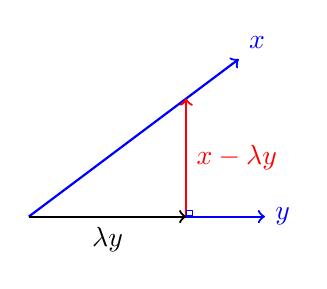
\begin{tikzpicture}[scale=0.5]
			\draw[blue, thick, ->] (0,0) -- (4+4/3,3+1) node[above right] {$x$};
			\draw[blue, thick, ->] (0,0) -- (6,0) node[right] {$y$};
			\draw[thick, red, ->] (4,0) -- (4,3) node[midway, right] {$x - \lambda y$};
			\draw[thick, ->] (0,0) -- (4,0) node[midway, below] {$\lambda y$};
			\draw[blue] (4.015,0.015) rectangle (4.15,0.15);

		\end{tikzpicture}
	\end{figure}
	¿Para qué $\lambda \in \R$, se tiene que  $\inner{y}{x-\lambda y } = 0$ ?

	\begin{align*}
		 & \leftrightarrow \inner{y}{x} - \lambda \inner{y}{y} = 0      \\
		 & \leftrightarrow \frac{\inner{y}{x}}{ \inner{y}{y}} = \lambda
	\end{align*}
	\begin{align*}
		\norm{x}^2 & = \norm{\lambda y +x-\lambda y}^2                                        \\
		           & =  \inner{xy+ x-\lambda y}{xy+ x-\lambda y}                              \\
		           & = \abs{\lambda}^2 \norm{y}^2+\underbrace{\norm{x-\lambda y}^2 }_{\geq 0}
	\end{align*}
	$$
		\rightarrow \norm{x}^2 \geq \abs{\lambda}^2 \norm{y}^2 = \frac{\abs{\inner{x}{y}}^2}{\norm{y}^2}
	$$
	$$
		\rightarrow \norm{x}^2 \norm{y}^2 \geq \abs{\inner{x}{y}}^2
	$$
	$$
		\rightarrow \norm{x}\norm{y} \geq \abs{\inner{x}{y}}, \quad \forall x,y \in \Rn
	$$
	Desigualdad de Cauchy-Schwarz.\\
	Además, la igualdad se da cuando uno de los vectores es multiplo del otro o $x, y$ es linealmente dependiente.
}

\clmp{}{
	$\forall\,  x, y \in \Rn, \norm{x+y} \leq \norm{x}+ \norm{y}$
}{
	Sean $x, y \in \Rn$
	\begin{align*}
		\norm{x+y}^2 & = \inner{x+y}{x+y}                                                     \\
		             & = \norm{x}^2+2\inner{x}{y}+\norm{y}^2                                  \\
		             & \leq  \norm{x}^2+2\norm{x}\norm{y}+\norm{y}^2  = (\norm{x}+\norm{y})^2
	\end{align*}
	$$
		\rightarrow \norm{x+y} \leq \norm{x}+\norm{y}
	$$
}


Dados $x,y \in \Rn, $   $d(x,y)=\norm{x-y}$
\begin{align*}
	d \colon \Rn \times \Rn & \longrightarrow \R                                                  \\
	(x,y)                   & \longmapsto d(x,y)= \norm{x-y}; \quad d(x,y) \text{ es una métrica}
\end{align*}

\begin{itemize}
	\item[(i)] $\forall \, x, y \in \Rn, d(x,y)\geq 0$
	\item[(ii)]  $\forall \, x, y \in \Rn, d(x,y) = d(y,x)  $ simetría
	\item[(iii)]   $\forall \,  x, y, z  \in \Rn, d(x,y) \leq d(x,z) + d(z,y)    $
	\item[(iv)]   $\forall \,  x, y   \in \Rn, d(x,z) =0 \, \leftrightarrow x=y  $
\end{itemize}


\ex{
	Sea $x = (x_1, \ldots, x_n) \in \Rn$,
	\begin{align}
		\norm{x}_1        & = \abs{x_1}+\abs{x_2}+\cdots +\abs{x_n} \label{eq:ex-norma-1} \\
		\norm{x}_{\infty} & = \max\{ \abs{x_1}, \abs{x_2}, \cdots, \abs{x_n}\} \nonumber  \\
		\norm{x}_2        & =\norm{x} = \sqrt{x_1^2+x_2^2+\cdots+ x_n^2} \nonumber
	\end{align}
	De \eqref{eq:ex-norma-1},
	\begin{align*}
		\norm{x+y}_1 & = \abs{x_1+y_1}+\cdots +\abs{x_n+y_n}                                          \\
		             & \leq \abs{x_1}+\abs{y_1}+\cdots + \abs{x_n}+\abs{y_n} =  \norm{x}_1+\norm{y}_1
	\end{align*}
	$$
		\norm{x} = \sqrt{x_1^2+\cdots x_1^n} \geq \abs{x_1} \rightarrow \norm{x}_{\infty} \leq \norm{x}
	$$
	$$
		\norm{x}_1 \geq \norm{x}
	$$
}

\clmp{Ley del paralelogramo}{

	Si $\norm{.} $ proviene de un producto interno en $\Rn$, entonces $\forall\, x,y \in \Rn$
	$$
		\norm{w} = \sqrt{\inner{w}{w}}
	$$
	$$
		\Rightarrow \norm{x+y}^2 +\norm{x-y}^2 = 2(\norm{x}^2+\norm{y}^2)
	$$
}{
	\begin{align}
		\norm{x+y}^2 = \inner{x+y}{x+y} = \norm{x}^2+2\inner{x}{y}+\norm{y}^2 \label{eq:paralelogramo-1} \\
		\norm{x-y}^2 = \inner{x+y}{x+y} = \norm{x}^2-2\inner{x}{y}+\norm{y}^2 \label{eq:paralelogramo-2}
	\end{align}

	De \eqref{eq:paralelogramo-1} y \eqref{eq:paralelogramo-2}
	$$
		\norm{x+y}^2 +\norm{x-y}^2 = 2(\norm{x}^2+\norm{y}^2)
	$$
}

\ex{
	En $\Real{2}, e_1=(1,0), e_2=(0,1)$\\
	Si $\norm{.}_1$ en $\Real{2}$ proviene de un producto interno.
	$$
		\rightarrow \forall \, x, y \in \Real{2}, \norm{x+y}_1^2 +\norm{x-y}_1^2 = 2(\norm{x}_1^2+\norm{y}_1^2)
	$$
	Si $x=e_1, \, y= e_2 \longrightarrow 2^2+2^2 = 2(1^2+1^2)$ (absurdo)\\
	Por lo tanto, $\norm{.}_1$ no proviene de un prducto interno.
}

Sean $\abs{.} \text{ y } \norm{.} $ dos normas en $\Rn$. Decimos que $\abs{.}$ y $\norm{.}$ son equivalentes si existen $\alpha, \beta \in \R^{+}$ tal que,
$$
	\forall\, x \in \Rn, \, \alpha \abs{x} \leq \norm{x}\leq\beta \abs{x}
$$

dada $\norm{.}$ norma en $\Rn$ la \textbf{BOLA ABIERTA } con centro en $a \in \Rn$ y radio $r>0$ es

$$
	B^{\norm{.}} (a,r) = \{z \in \Rn\colon \norm{z-a} < r\}
$$

En $\Real{2}$

$$
	B^{\norm{.}} (\Ou,1) = \{(z_1, z_2) \in \Real{2} \colon \norm{(z_1, z_2)} < 1\}
$$

\begin{figure}[H]
	\centering
	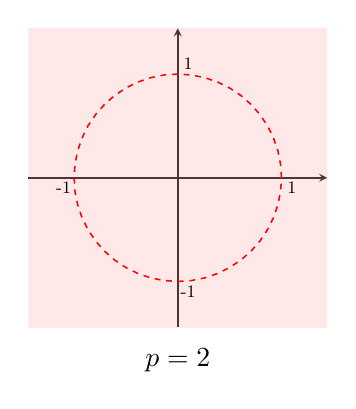
\begin{tikzpicture}[scale=0.7]
		\begin{axis}[
				width=7cm, height=7cm,
				axis lines=middle,
				xtick=\empty, ytick=\empty,
				axis equal,
				enlargelimits,
				xmin=-1.2, xmax=1.2,
				ymin=-1.2, ymax=1.2,
				thick,
				domain=0:90
			]

			\draw [fill = red!30, opacity=0.3, draw=none]  (axis cs:0,0) circle[radius=100];

			%p=2
			\addplot[red,domain=-pi:0,  thick, dashed] ({(cos(deg(x)))},{(sin(deg(x))});
			\addplot[red,domain=0:pi,  thick, dashed] ({(cos(deg(x)))},{(sin(deg(x))});


			% Add +1 and -1 labels
			\node[font=\small] at (axis cs:1.1,-0.1) {1};
			\node[font=\small] at (axis cs:-1.1,-0.1) {-1};
			\node[font=\small] at (axis cs:0.1,1.1) {1};
			\node[font=\small] at (axis cs:0.1,-1.1) {-1};

		\end{axis}
		\node[below=0.5cm, anchor=base] at (current axis.south) {$p=2$}; % Print p
	\end{tikzpicture}
\end{figure}
$$
	B^{\norm{.}_{\infty}} (\Ou,1) = \{(z_1, z_2) \in \Real{2} \colon \max{\abs{z_1}, \abs{z_2}} < 1\}
$$
\begin{figure}[H]
	\centering
	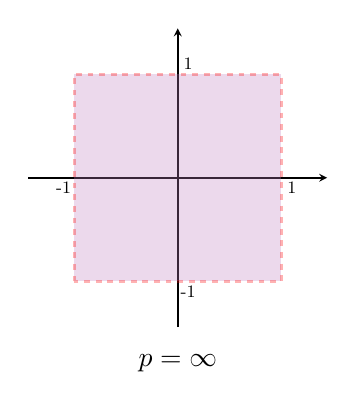
\begin{tikzpicture}[scale=0.7]
		\begin{axis}[
				width=7cm, height=7cm,
				axis lines=middle,
				xtick=\empty, ytick=\empty,
				axis equal,
				enlargelimits,
				xmin=-1.2, xmax=1.2,
				ymin=-1.2, ymax=1.2,
				thick,
				domain=0:90
			]

			%p=inf
			\draw[ultra thick, dashed, red!100!blue, fill=red!50!blue!50, opacity=0.3,] (axis cs:-1,-1) rectangle (axis cs:1,1);

			% Add +1 and -1 labels
			\node[font=\small] at (axis cs:1.1,-0.1) {1};
			\node[font=\small] at (axis cs:-1.1,-0.1) {-1};
			\node[font=\small] at (axis cs:0.1,1.1) {1};
			\node[font=\small] at (axis cs:0.1,-1.1) {-1};

		\end{axis}
		\node[below=0.5cm, anchor=base] at (current axis.south) {$p=\infty$}; % Print p
	\end{tikzpicture}
\end{figure}



$$
	B^{\norm{.}_{1}} (\Ou,1) = \{(z_1, z_2) \in \Real{2} \colon   \abs{z_1}+ \abs{z_2}< 1\}
$$

\begin{figure}[H]
	\centering
	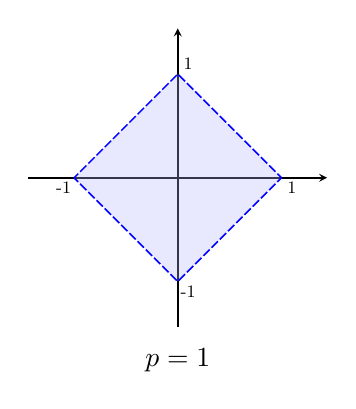
\begin{tikzpicture}[scale=0.7]
		\begin{axis}[
				width=7cm, height=7cm,
				axis lines=middle,
				xtick=\empty, ytick=\empty,
				axis equal,
				enlargelimits,
				xmin=-1.2, xmax=1.2,
				ymin=-1.2, ymax=1.2,
				thick,
				domain=0:90
			]

			\addplot  [fill=blue!30, opacity=0.3, draw=none] coordinates { (0,1) (-1,0) (0,-1) (1,0)}
			--cycle;


			\foreach \sx in {1,-1} {
					\foreach \sy in {1,-1} {
							\addplot[blue, domain=0:pi,  thick, dashed]
							({\sx*(cos(deg(x)))^2}, {\sy*(sin(deg(x)))^2});
						}
				}

			% Add +1 and -1 labels
			\node[font=\small] at (axis cs:1.1,-0.1) {1};
			\node[font=\small] at (axis cs:-1.1,-0.1) {-1};
			\node[font=\small] at (axis cs:0.1,1.1) {1};
			\node[font=\small] at (axis cs:0.1,-1.1) {-1};

		\end{axis}
		\node[below=0.5cm, anchor=base] at (current axis.south) {$p=1$}; % Print p
	\end{tikzpicture}
\end{figure}



\thmr{ Equivalencia de normas en $\Rn$ }{teorema1}{

	En $\Rn$ todas las normas son equivalentes.
}

\pf{ del   Theorem~\ref{thm:teorema1}\\
	Sea $(x_k)_{k \in \N}$ una sucesión de puntos de $\Rn$
	\begin{align*}
		x \colon \N & \longrightarrow \Rn                                   \\
		k           & \longmapsto x(k)= x_k = (x_1^k, x_2^k, \ldots, x_n^k)
	\end{align*}
	Sea $a = (a_1, a_2, \ldots, a_n) \in \Rn $, decimos que $(x_k)_{k \, \in \, \N} $ converge a $a \, \in \Rn$ si,

	$$
		\forall\, \varepsilon >0, \exists k_0 \in \, \N, \forall \, k \in \N , k \geq k_0 \longrightarrow \norm{x_k-a} <\varepsilon
	$$
	$$
		\lim\limits_{k \to \infty} x_k =a \text{ es respecto a la norma  }\quad \norm{x_k-a}_{\infty} \leq \abs{(x_k-a)}
	$$

}


\rmkb{
	$$
		\norm{x}_{\infty} \leq \norm{x} \leq \norm{x}_1 \leq n\norm{x}_{\infty}\leq n \norm{x}_1
	$$
	$$
		\Rightarrow \norm{x} \leq \norm{x}_1 \leq n \norm{x}
	$$
}


\thmr{Criterio de convergencia en \(\mathbb{R}^n\)}{teorema2}{
	Sea \((x_k)_{k \in \mathbb{N}} \subset \mathbb{R}^n\), donde
	\[
		x_k = (x_1^k, x_2^k, \ldots, x_n^k) \quad \forall\, k \in \mathbb{N},
	\]
	y sea \(a = (a_1, a_2, \ldots, a_n) \in \mathbb{R}^n\).

	Entonces,
	\[
		\lim_{k \to \infty} x_k = a \quad \text{si y solo si} \quad \forall\, i \in \{1, \ldots, n\},\; \lim_{k \to \infty} x_i^k = a_i.
	\]
}

\pf{ del teorema \ref{thm:teorema2} \\
	$(\Rightarrow)$ Supongamos que $\lim\limits_{k\to \infty} x_k =a$\\
	Dado,
	$
		\varepsilon > 0, \exists\, k_0 \in \N, \forall\, k \in \N
	$

	$$
		k\geq k_0 \longrightarrow \abs{x_i^k-a} \leq  \norm{x_k-a}_{\infty} \leq \norm{x_{k}-a} < \varepsilon, \quad \forall \, i \in \{1, \ldots, n\}
	$$
	$$
		\therefore  \lim\limits_{k\to \infty} x_i^k =a_i,\quad \forall\, i \in \{1, \ldots, n\}
	$$

	$(\Leftarrow)$ Suponga que $\forall \, i \in \{1,\ldots, n\}$

	$$
		\lim\limits_{k\to \infty} x_i^k =a_i
	$$
	Dado $\varepsilon >0, \forall\, i \in \{1,\ldots, n\} \, \exists \, k_i^o \in \N$ tal que $\forall \, k \in \N, \varepsilon_0 =\frac{\varepsilon}{\sqrt{n}}$


	\begin{align*}
		k \geq k_i^o & \rightarrow \abs{x_i^k -a_i} < \varepsilon_0     \\
		             & \rightarrow \abs{x_i^k -a_i}^2 < \varepsilon_0^2
	\end{align*}
	Sea $k_0 = \max \{k_1^0,\, k_2^0, \ldots, \,k_n^0\}$ si $	k \geq k_0 \geq k_i^0  \; \forall\; i \in \{1, 2, \ldots, n\}$

	$$
		\rightarrow \sqrt{\sum_{i=1}^{n}\abs{x_i^k-a_i}^2}< \sqrt{n \varepsilon_0^2}
	$$
	$$
		\rightarrow \norm{x_i^k -a} < \sqrt{n} \varepsilon_0 =\varepsilon
	$$

	%Theorem~\ref{{thm:Teorema1}

}



























